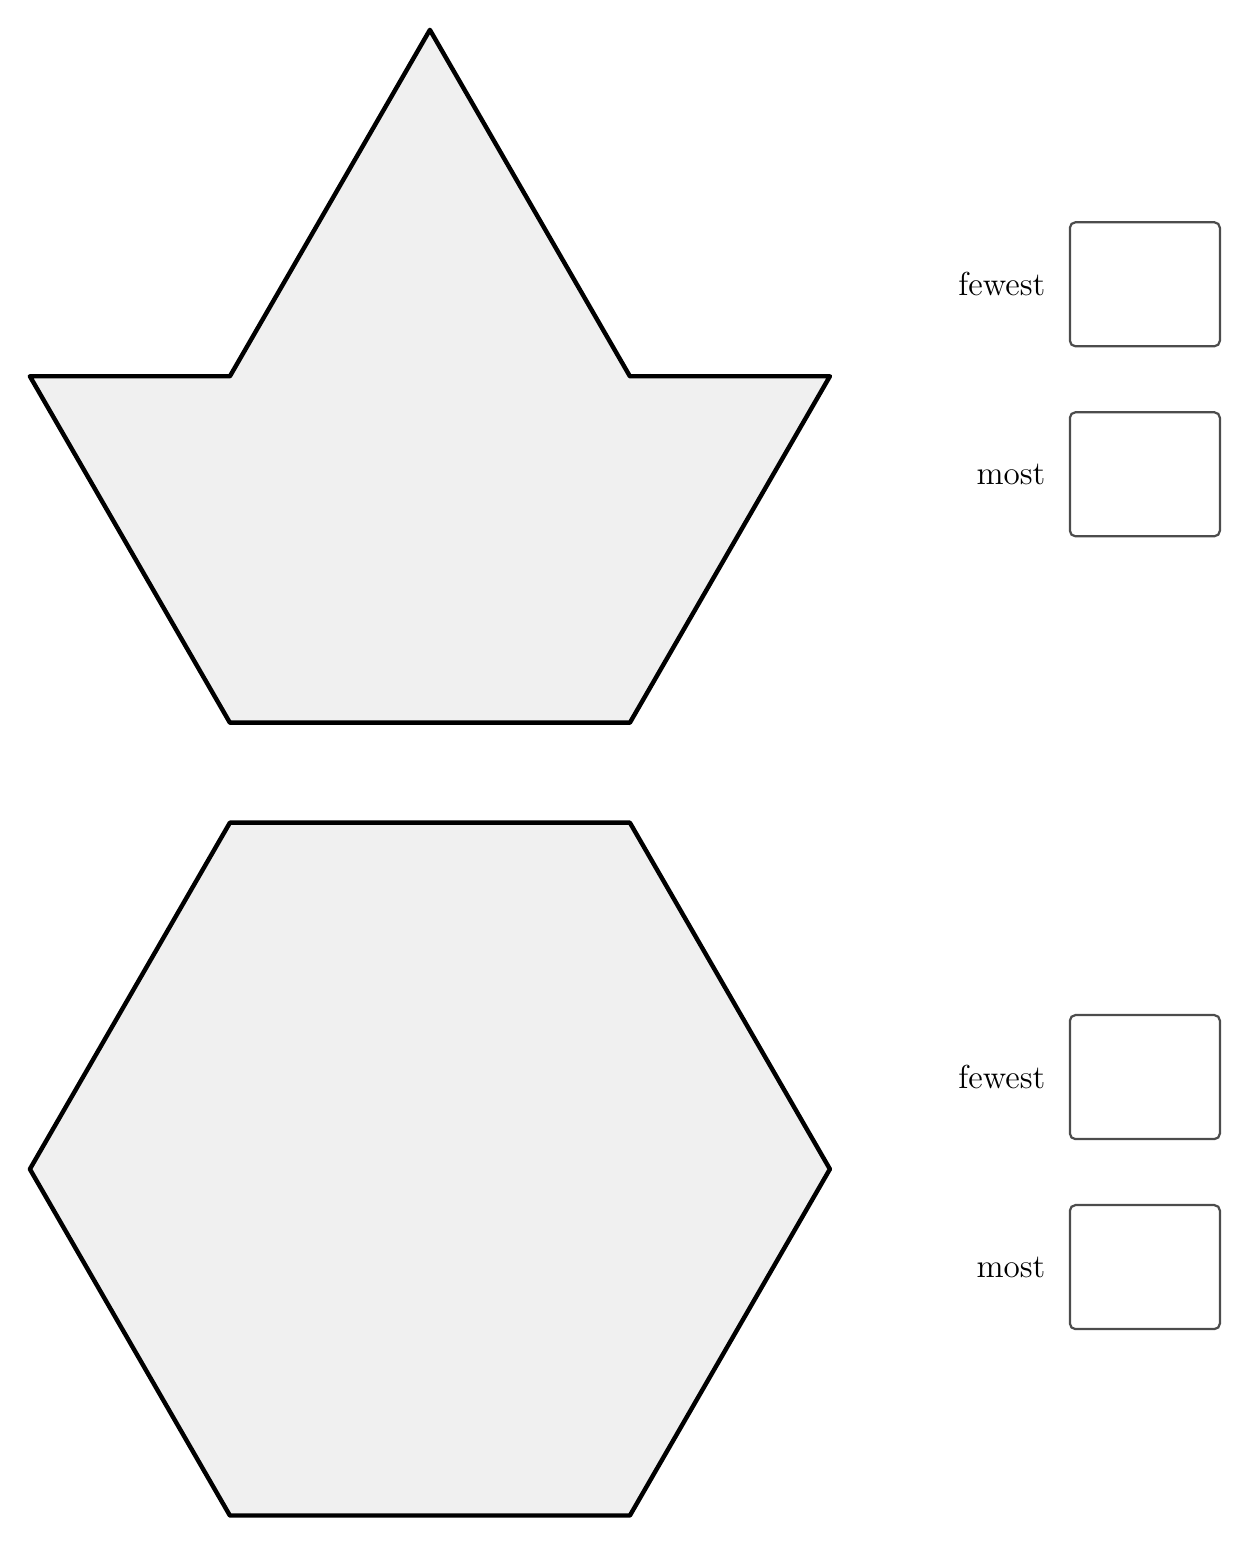
\begin{tikzpicture}[x=1in,y=1in]
\fill[black!6, even odd rule] (0.8,1.7321) -- (1.8,0) -- (3.8,0) -- (4.8,1.7321) -- (3.8,3.4641) -- (1.8,3.4641) -- cycle;
\draw[line width=1.6pt, black, line join=round] (0.8,1.7321) -- (1.8,0) -- (3.8,0) -- (4.8,1.7321) -- (3.8,3.4641) -- (1.8,3.4641) -- cycle;
\node[anchor=east, inner sep=0pt] at (5.88,1.2421) {\large most};
\draw[line width=0.8pt, black!70, rounded corners=2pt] (6,0.9321) rectangle (6.75,1.5521);
\node[anchor=east, inner sep=0pt] at (5.88,2.1921) {\large fewest};
\draw[line width=0.8pt, black!70, rounded corners=2pt] (6,1.8821) rectangle (6.75,2.5021);
\fill[black!6, even odd rule] (1.8,5.6962) -- (0.8,5.6962) -- (1.8,3.9641) -- (3.8,3.9641) -- (4.8,5.6962) -- (3.8,5.6962) -- (2.8,7.4282) -- cycle;
\draw[line width=1.6pt, black, line join=round] (1.8,5.6962) -- (0.8,5.6962) -- (1.8,3.9641) -- (3.8,3.9641) -- (4.8,5.6962) -- (3.8,5.6962) -- (2.8,7.4282) -- cycle;
\node[anchor=east, inner sep=0pt] at (5.88,5.2062) {\large most};
\draw[line width=0.8pt, black!70, rounded corners=2pt] (6,4.8962) rectangle (6.75,5.5162);
\node[anchor=east, inner sep=0pt] at (5.88,6.1562) {\large fewest};
\draw[line width=0.8pt, black!70, rounded corners=2pt] (6,5.8462) rectangle (6.75,6.4662);
\end{tikzpicture}
